\documentclass[paper=letter, fontsize=11pt]{scrartcl} % A4 paper and 11pt font size
\usepackage{graphicx}
\usepackage{enumitem}
\usepackage{listings,multicol}
\usepackage[T1]{fontenc} % Use 8-bit encoding that has 256 glyphs
\usepackage{fourier} % Use the Adobe Utopia font for the document - comment this line to return to the LaTeX default
\usepackage[english]{babel} % English language/hyphenation
\usepackage{amsmath,amsfonts,amsthm} % Math packages
\usepackage{lipsum} % Used for inserting dummy 'Lorem ipsum' text into the template
\usepackage{sectsty} % Allows customizing section commands
\allsectionsfont{\centering \normalfont\scshape} % Make all sections centered, the default font and small caps
\usepackage{fancyhdr} % Custom headers and footers
\pagestyle{fancyplain} % Makes all pages in the document conform to the custom headers and footers
\fancyhead{} % No page header - if you want one, create it in the same way as the footers below
\fancyfoot[L]{} % Empty left footer
\fancyfoot[C]{} % Empty center footer
% \fancyfoot[R]{\thepage} % Page numbering for right footer
\renewcommand{\headrulewidth}{0pt} % Remove header underlines
\renewcommand{\footrulewidth}{0pt} % Remove footer underlines
\setlength{\headheight}{13.6pt} % Customize the height of the header

\setlength\parindent{0pt} % Removes all indentation from paragraphs - comment this line for an assignment with lots of text

\usepackage[margin=0.75in]{geometry}
\usepackage{hyperref}
%----------------------------------------------------------------------------------------
%   TITLE SECTION
%----------------------------------------------------------------------------------------

\newcommand{\horrule}[1]{\rule{\linewidth}{#1}} % Create horizontal rule command with 1 argument of height

\title{ 
    \normalfont \normalsize 
    \textsc{CS 3060 Programming Languages, Fall 2020} \\ [25pt] % Your university, school and/or department name(s)
    \horrule{0.5pt} \\[0.4cm] % Thin top horizontal rule
    \huge Assignment \#6  \\ % The assignment title
    \horrule{2pt} \\[0.5cm] % Thick bottom horizontal rule
}

% \author{John Smith} % Your name

% \date{\normalsize\today} % Today's date or a custom date

\begin{document}

    \begin{center}
         Assignment \#6\\
        \small CS 3060 Programming Languages, Fall 2020 \\
        \small Instructor: S. Roy \\
        \huge Scala \#2
    \end{center}
    
    \textbf{Due Date:} November 8 @ 11.59 PM. \\
    \textbf{Total Points:} 60 points \\

    \textbf{Directions:} Using the source provided via Gitlab \@ \texttt{https://gitlab.com/sanroy/fa20-cs3060-hw/},
complete the assignment below. The process for completing this assignment should be as follows:

    \begin{enumerate}[noitemsep]
        \item You already forked the Repository ``sanroy/fa20-cs3060-hw'' to a repository ``yourId/fa20-cs3060-hw'' under your username. If not, do it now.
        \item Get a copy of hw6 folder in ``sanroy/fa20-cs3060-hw'' repository as a hw6 folder in your repository ``yourId/fa20-cs3060-hw''
        \item Complete the assignment, committing changes to git. Each task code should be in a separate file. As an example, task1.scala for Task 1.
        \item Push all commits to your Gitlab repository
        \item If you have done yet done so, sdd TA (username: prabeshpaudel) as a member of your Gitlab repository
    \end{enumerate}


    \textbf{Tasks:}
    \begin{enumerate}
       \item \textbf{(15 points) Task \#1:} In this task, your code creates a random list of 50 shape objects, 
then traverses the list from start to end, and computes the total area of the shape objects. 
First you need to implement the class hierarchy diagram of the shape types, which is aavailable in the same directory. 
Shape is an abstract class which has only a "color" attribute whereas Circle class and Rectangle class are concrete 
children of Shape class, and they have more attributes and constructors. 
Note that you do not know beforehand the order of the shape objects (i.e. Circles and Rectangles) 
created in the random list, e.g. you do not know beforehand whether the 1st item is Circle or Rectangle.
\emph{Writing README carries 1 point.}

Note. When you traverse the list to calculate the total area, you need to call the area() function of each shape object.

\textbf{Hint:} While building the list of shape objects, generate a random number 0 or 1; if 0, then you may add a Circle object, else add a Rectangle object to the list.

\begin{figure}
  \centering
  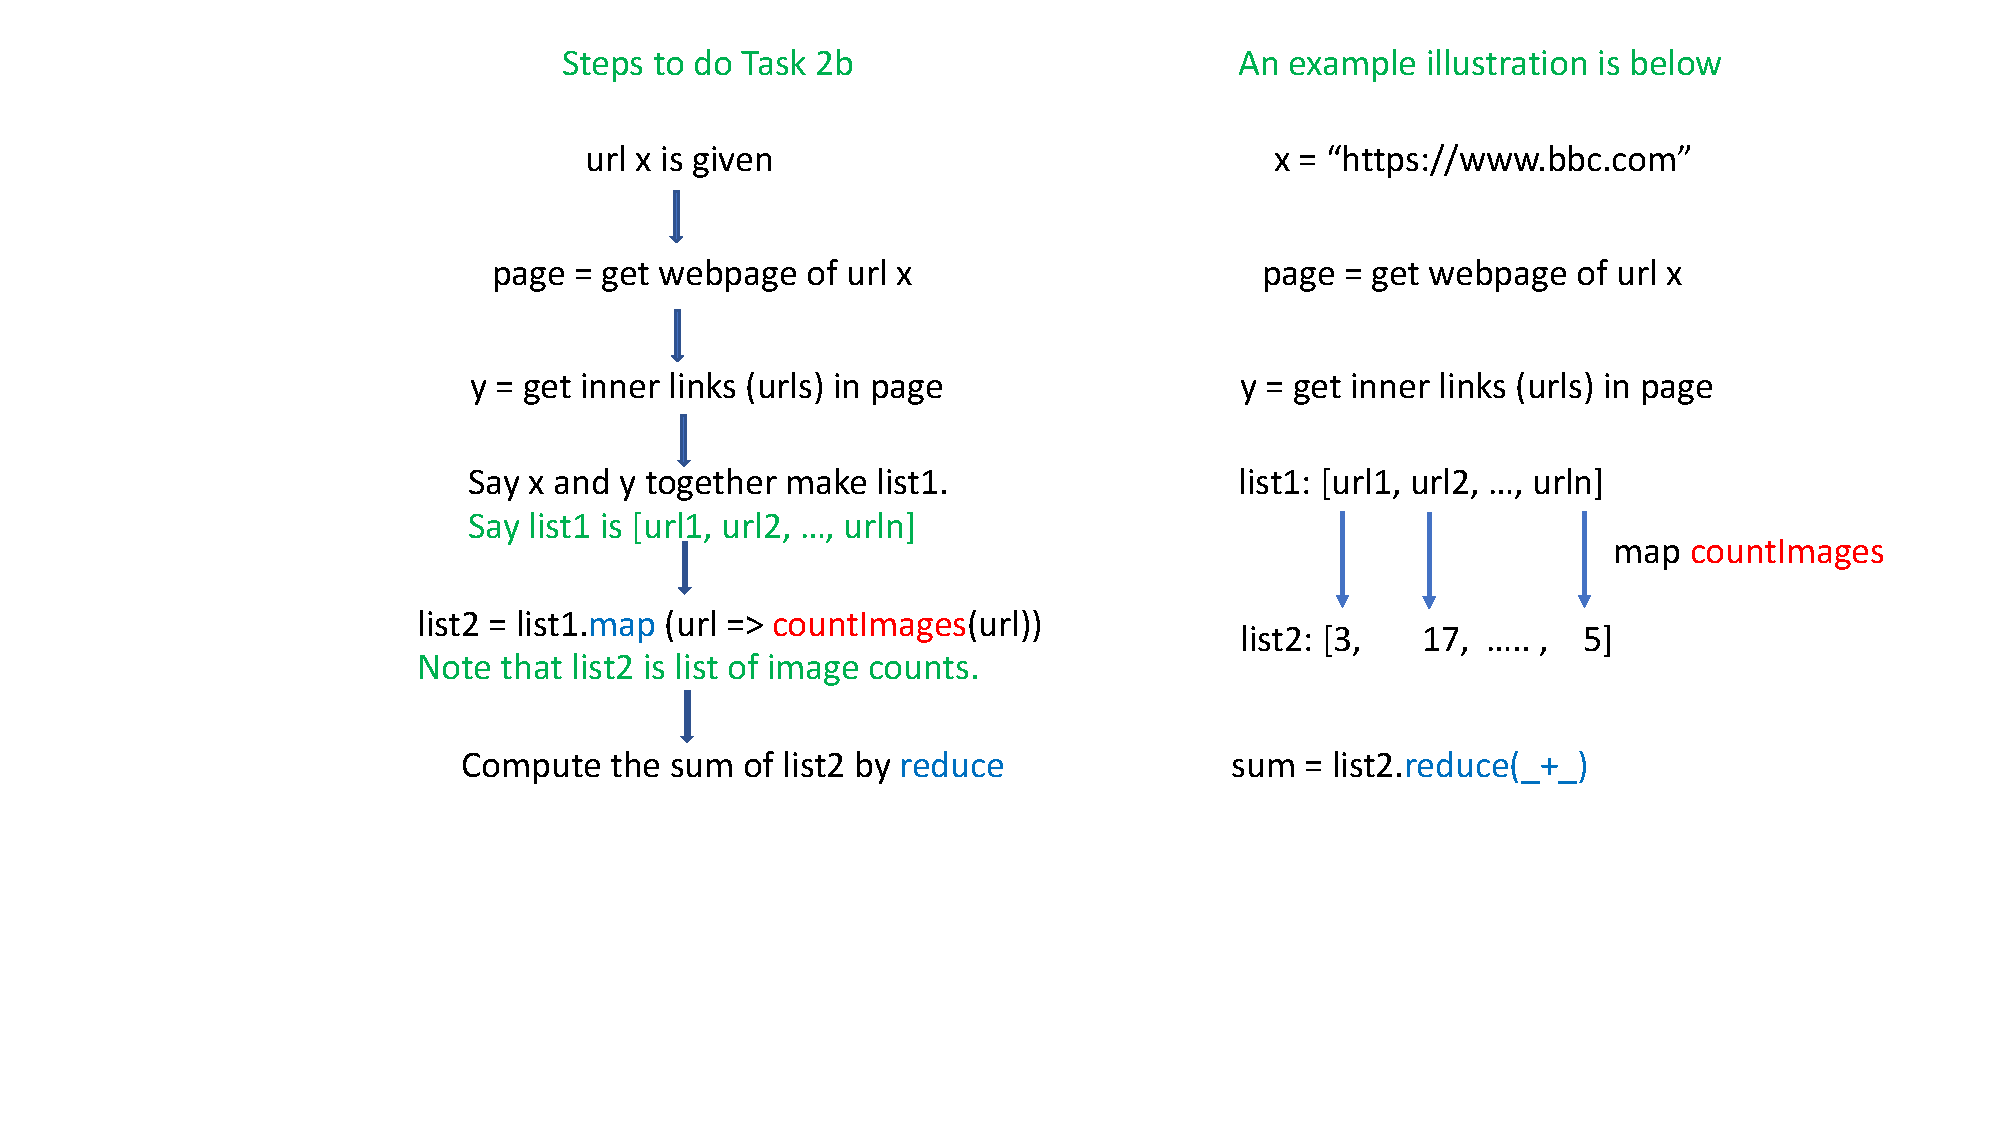
\includegraphics[width=15cm]{task2Fig.pdf}
  \caption{The steps to do for Task 2b.}  \label{fig:2b}
\end{figure}

        \item \textbf{Task \#2a: (8 points)} Write a Scala program which takes a webpage url (say x) from the user, and then download webpage x.
Count the number of images (i.e. "<img .../>") and scripts (i.e. "<script ...> </script>") present in x.


        \textbf{Task \#2b: (8 points)} Say webpage x contains links to other webpages (can be zero, one, or more) y.
Your program needs to download all such pages (i.e. x and y). Count the total num of images on x and y. See Figure~\ref{fig:2b}.

        \textbf{Task \#2c: (7 points)} Also, your program needs to count how many pages (found in Task 2b) have more than 2 images.

        \textbf{Task \#2d: (7 points)} Do Task 2b again, but now you are using the \texttt{par} (i.e. parallel collection).
How much time does the concurrency usage save compared to the serial run in Task 2b?

\emph{Writing README for Task 2 carries 2 points.}

\newpage

        \item \textbf{Task \#3a: (10 points)} Write a function foo which takes a list t of strings as input. 
        For each string s in t, foo uses the higher-order function \texttt{map} to compute the list of unique characters present in string s. Finally, foo returns a new list containing these lists. As an example, if t is ["abcdb", "bcdd"], then foo should return [['a', 'b', 'c', 'd'], ['b', 'c', 'd']].

        \textbf{Task \#3b: (5 points)} Write a function foo which takes a list t of integers as input. 
        Then, foo uses \texttt{foldLeft} to compute the sum of cubes of all elements of t. Finally, foo returns the computed sum.

\emph{Writing README for Task 3 carries 1 point.}

    % \vspace{2cm}
    
    \end{enumerate}

\end{document}


